\documentclass[t]{beamer}

\setlength {\marginparwidth }{2cm}
\setlength {\parskip}{0cm}
\usepackage{todonotes}
\usepackage{siunitx}
\usepackage{subcaption}
\usepackage{apacite}    % Use APA Citation
\presetkeys{todonotes}{inline}{}
\beamertemplatenavigationsymbolsempty
\usefonttheme[onlymath]{serif}

\usepackage{algpseudocode}
\usepackage{enumitem,amssymb, yfonts, bm}
\newlist{todolist}{itemize}{2}
\setlist[todolist]{label=$\square$}
\usepackage{pifont}
\newcommand{\cmark}{\ding{51}}%
\newcommand{\xmark}{\ding{55}}%
\newcommand{\done}{\rlap{$\square$}{\raisebox{2pt}{\large\hspace{1pt}\cmark}}%
\hspace{-2.5pt}}

% \usetheme{AnnArbor}
% \usetheme{Antibes}
% \usetheme{Bergen}
% \usetheme{Berkeley}https://www.sharelatex.com/project/5b12e1a4f84b363f6f336dab
% \usetheme{Berlin}
% \usetheme{Boadilla}
% \usetheme{boxes}
\usetheme{CambridgeUS}
% \usetheme{Copenhagen}
%\usetheme{Darmstadt}
% \usetheme{default}
%\usetheme{Frankfurt}
%\usetheme{Goettingen}
% \usetheme{Hannover}
% \usetheme{Ilmenau}
% \usetheme{JuanLesPins}
\setlength{\parskip}{10pt}

% \newcommand*\vc[1]%
% {\begin{pmatrix}#1\end{pmatrix}}

\newcommand*\vc[1]%
{\left(\begin{array}{cccc}#1\end{array}\right)}


\newcommand\eqdef{\ \mathrel{\overset{\makebox[0pt]{\mbox{\normalfont\scriptsize\rmfamily def}}}{=}}\ }

\title[Eligibility propagation]{Eligibility propagation in multi-layer recurrent spiking neural networks.\\\vspace{10pt}
\large{Presentation 10: Evaluation meeting 2}}

\author[Werner van der Veen]{Werner~van~der~Veen\\\footnotesize\texttt({w.k.van.der.veen.2@student.rug.nl})}\date{\today}

\begin{document}

\begin{frame}
    \titlepage
\end{frame}

%======================================

% \begin{frame}
%    \tableofcontents
% \end{frame}

\small

\section{Abstract}

\section{Introduction}
  \begin{frame}{Introduction -- context}
    \begin{itemize}[label=--]
      \item Biological inspiration to AI
      \item ANNs and backpropagation
      \item Deep learning
    \end{itemize}

  \end{frame}

  \begin{frame}{Introduction -- relevance}
    \begin{itemize}[label=--]
      \item Deep learning is energy intensive
      \item Fundamental differences between DL and biological learning
      \item
      \begin{itemize}[label=--]
        \item Continuous vs. binary communication
        \item Backpropagation/BPTT vs. learning signals
      \end{itemize}
    \end{itemize}

  \end{frame}

  \begin{frame}{Introduction -- SNNs}
    \begin{itemize}[label=--]
      \item Binary spikes $\rightarrow$ no backpropagation
      \item Good performance, but not competitive with DL

    \begin{figure}[!ht]
      \centering
      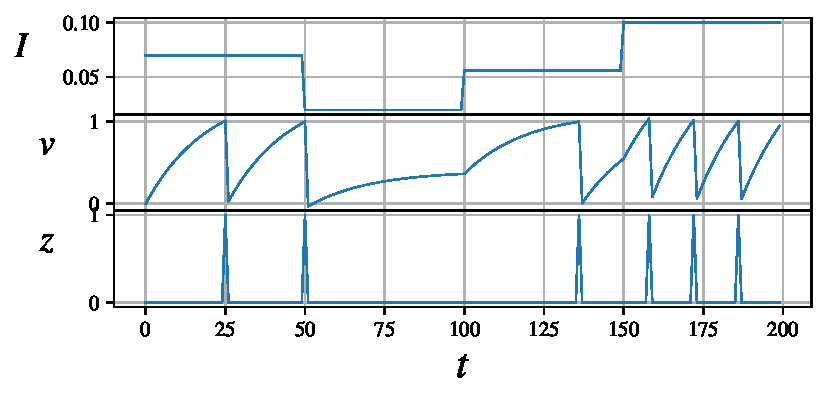
\includegraphics[width=\linewidth]{simplesnn}
    \end{figure}
    \end{itemize}
  \end{frame}

  \begin{frame}{Introduction -- neuromorphic computing}
    \begin{itemize}[label=--]
      \item Physical embedding of neural network in an analog medium
      \item Colocalized memory and computation \\$\rightarrow$ no backpropagation
      \item SNNs as ideal biologically inspired NC paradigm for efficient computation
      \item Analog SNNs are extremely fast and energy efficient
      \item Problem: learning rule must be \emph{local} and \emph{online}\\$\rightarrow$ revalue biological learning
    \end{itemize}

  \end{frame}

  \begin{frame}{Introduction -- biological learning}
    \begin{itemize}[label=--]
      \item Hebbian learning \\$\rightarrow$ runaway excitation
      \item STDP \\$\rightarrow$ how to teach?
      \item Learning signals: three-factor Hebbian learning, R-STDP
      \item Biological learning signals: neurotransmitters\\$\rightarrow$ credit assignment
      \item Eligibility traces
    \end{itemize}
  \end{frame}

  \begin{frame}{Introduction -- eligibility propagation}
    \begin{itemize}[label=--]
      \item Mathematical approximation to BPTT
      \item Local learning signals and eligibility traces
      \item Applicable to any SNN topology and multiple neuron models
      \item Also applicable to neuromorphic VLSIs
      \item Competitive with LSTMs on phone classification
    \end{itemize}
  \end{frame}

  \begin{frame}{Introduction -- eligibility propagation}
    \begin{itemize}[label=--]
      \item E-prop: only ALIF so far
      \item New research: STDP-LIF and Izhikevich neuron display STDP
    \end{itemize}
  \end{frame}

  \begin{frame}{Introduction -- this research}
    \begin{itemize}[label=--]
      \item Reproduce results of original e-prop paper\\$\rightarrow$ explicitly instead of automatic differentiation
      \item Extend STDP-LIF to STDP-ALIF
      \item Experimentally verify the STDP-ALIF and Izhikevich neuron on phone classification task
      \item Examine effects of e-prop in multi-layer recurrent SNN
    \end{itemize}
  \end{frame}

\section{Methods}
\begin{frame}{Methods -- technical framework (e-prop)}

  \begin{figure}[!ht]
    \centering
    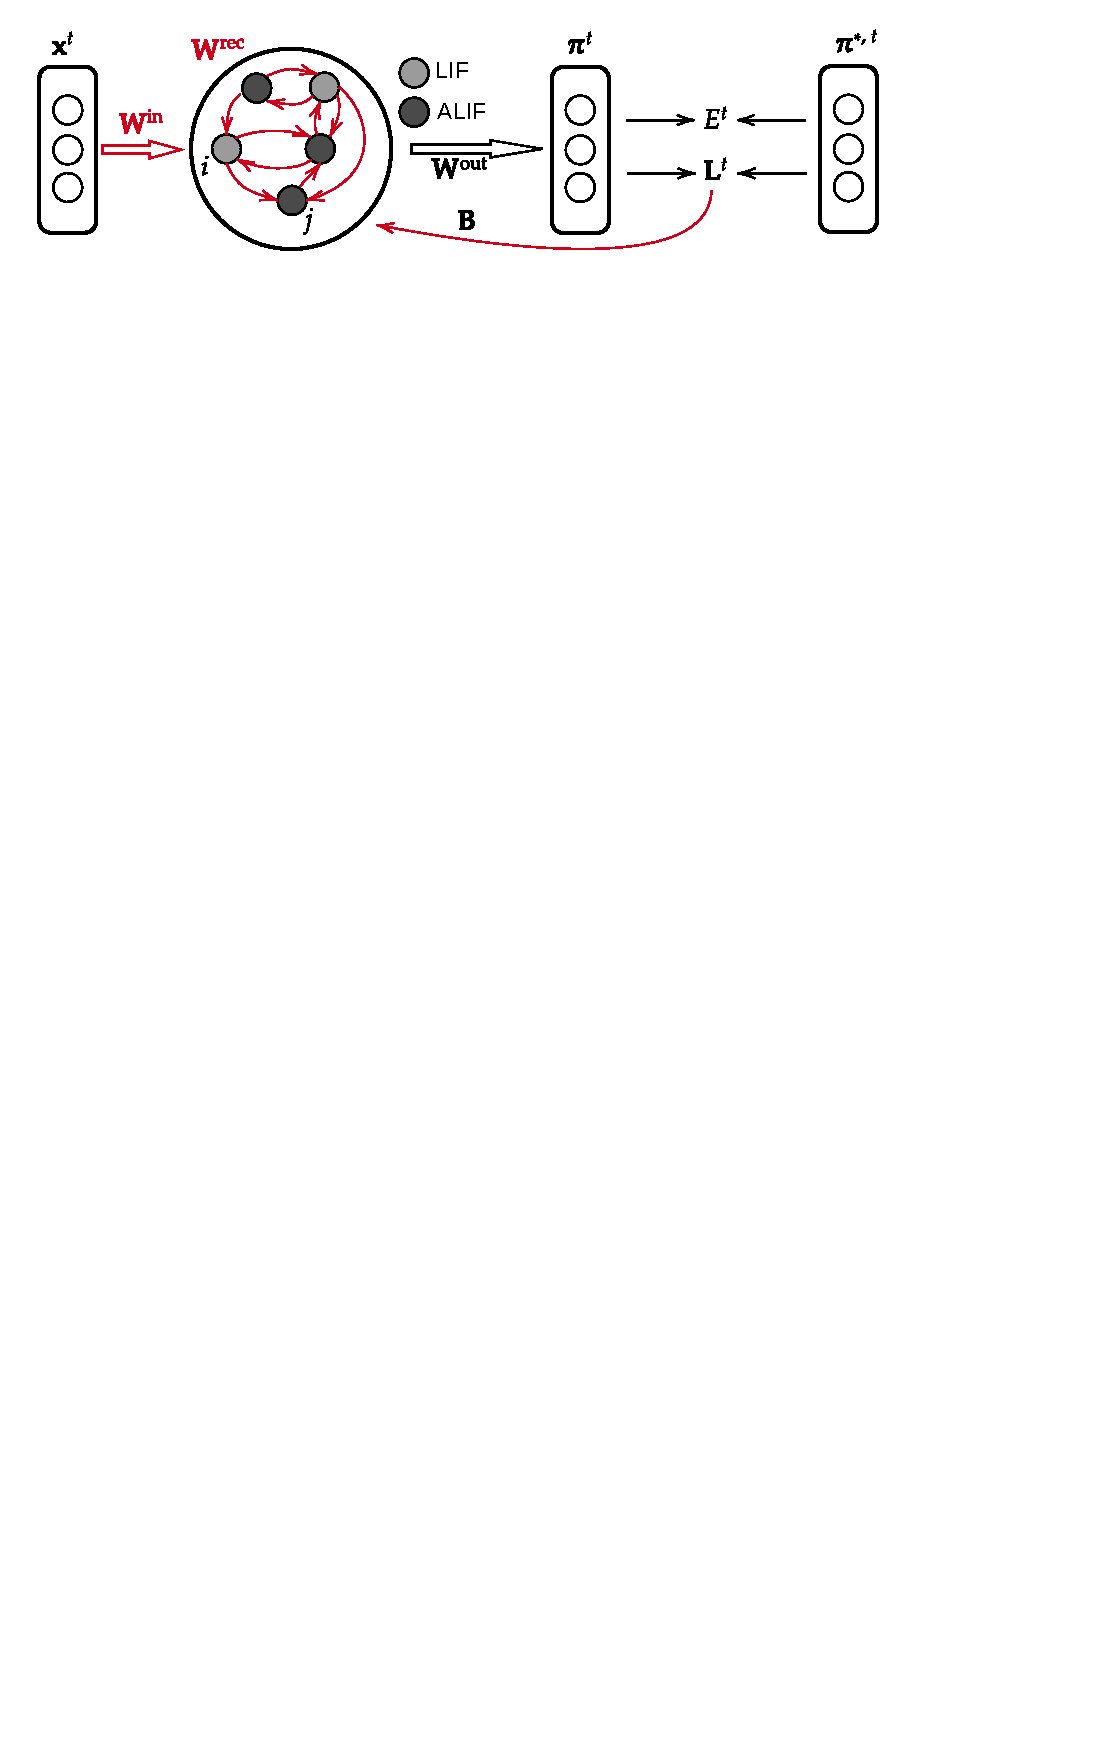
\includegraphics[trim=0 25cm 0 0, clip, width=\linewidth]{Singlelayer}
  \end{figure}
  E-prop model $\mathcal{M} = \left<M, f\right>$
  \begin{equation}\label{eq:model}
    \mathbf{h}^t_j = M\left(\mathbf{h}_j^{t-1}, \mathbf{z}^{t-1}, \mathbf{x}^t, \mathbf{W}_j\right)
  \end{equation}
  \begin{equation}
  z^t_j = f\left(\mathbf{h}_j^t\right)
  \end{equation}
  % Local and online!
\end{frame}

\begin{frame}{Methods -- the ALIF neuron model}
  \begin{figure}[!ht]
    \centering
    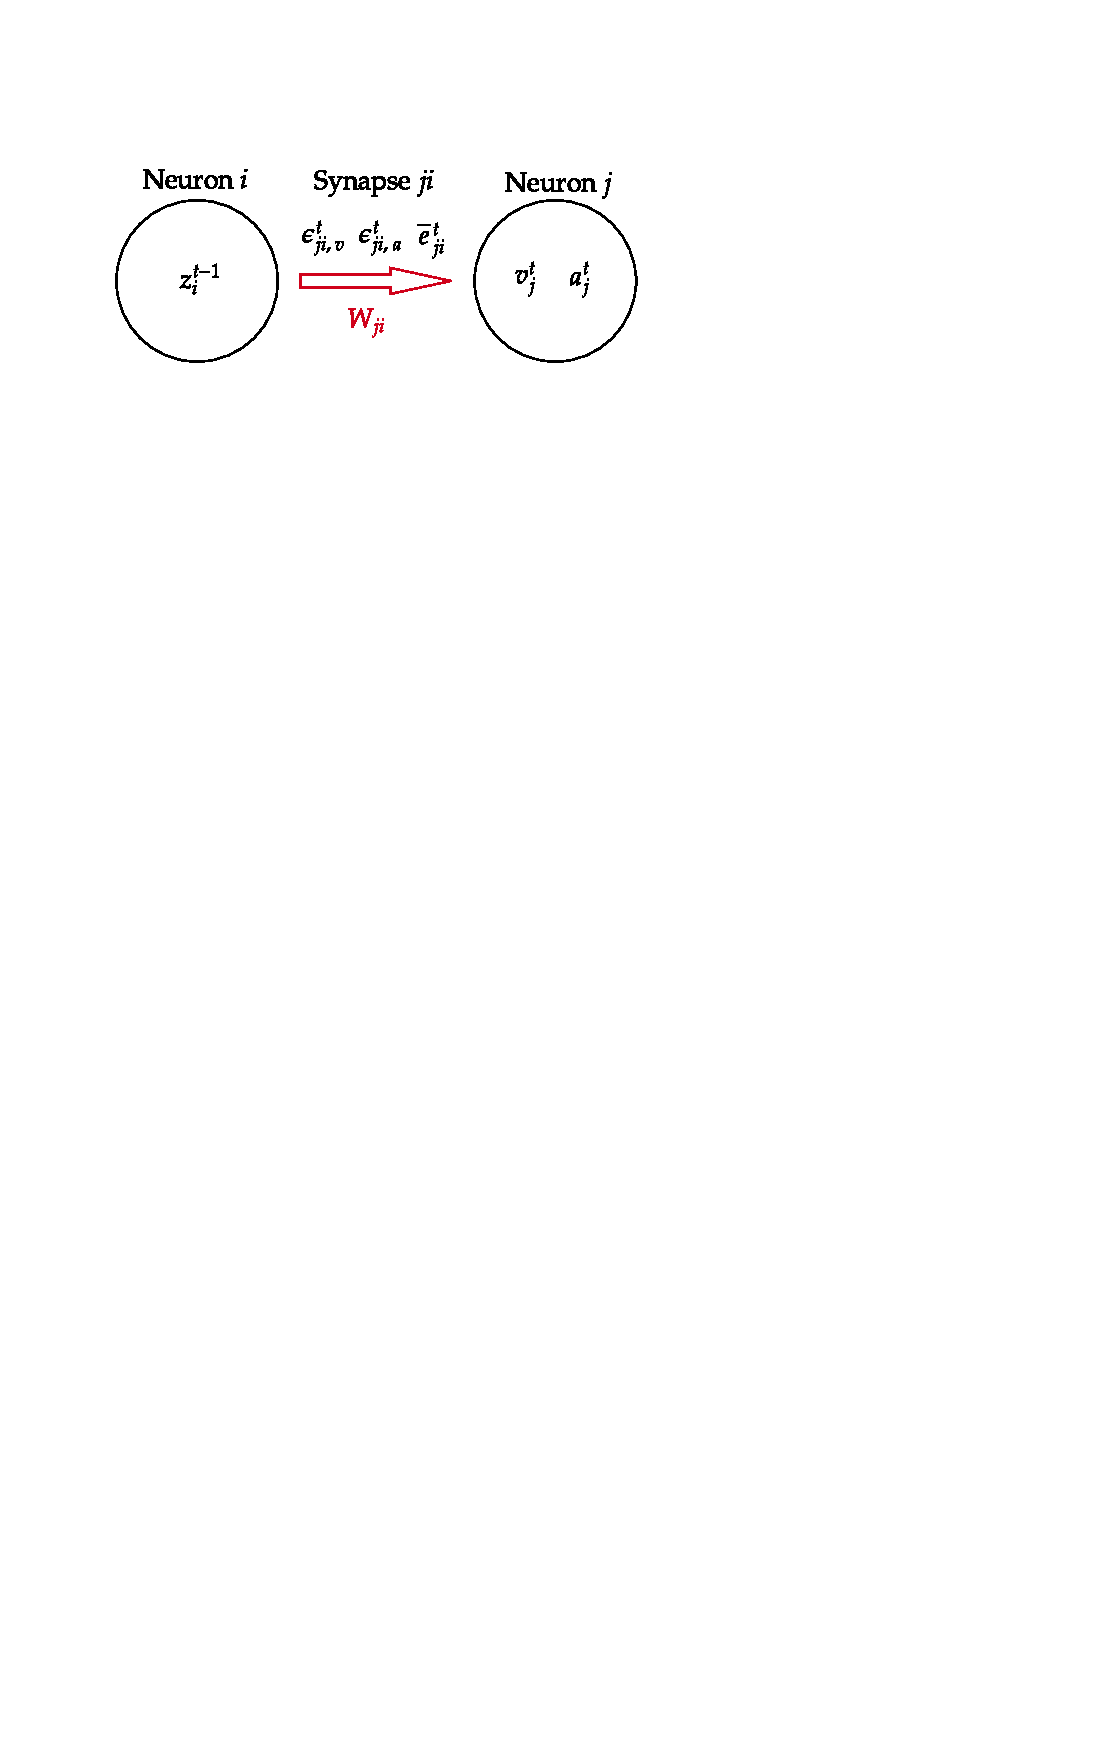
\includegraphics[width=\linewidth]{Neuron}
  \end{figure}
  \begin{figure}[!ht]
    \centering
    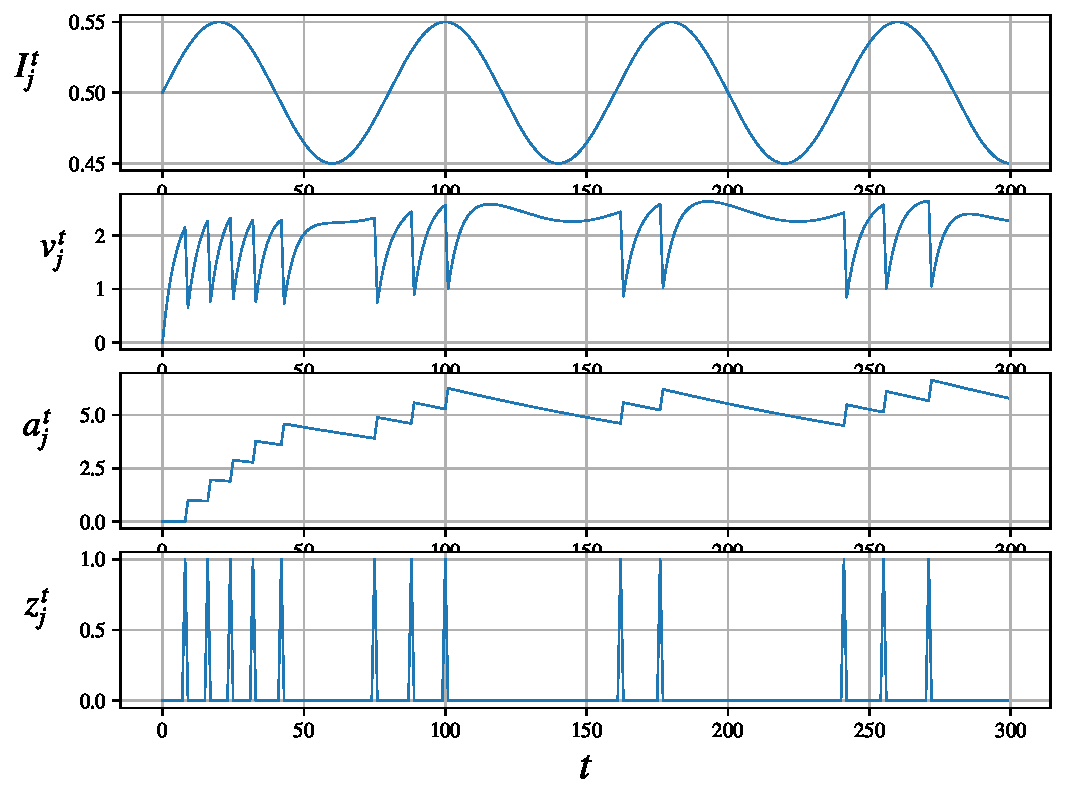
\includegraphics[width=\linewidth]{simplealif}
  \end{figure}
\end{frame}

\begin{frame}{Methods -- the ALIF neuron model}
  \begin{equation}
  z^t_j = H\left(v_j^t - v_\text{th} - \beta a^t_j\right)
  \end{equation}
  \begin{equation}\label{eq:alifV}
  v^{t+1}_j = \alpha v_j^t + \sum_{i\neq j}W^\text{rec}_{ji}z_i^t + \sum_i W^\text{in}_{ji}x_i^{t+1} - z_j^tv_
  \text{th}
  \end{equation}
  \begin{equation}\label{eq:alifA}
  a^{t+1}_j = \rho a^t_j + z^t_j
  \end{equation}
  % 25% is LIF, so effectively beta = 0
\end{frame}

\begin{frame}{Methods -- e-prop}
  \begin{align*}
    \frac{dE}{dW_{ji}} &= \sum_tL^t_j\ e^t_{ji}\\
    \frac{dE}{dW_{ji}} &= \sum_t\frac{dE}{dz_j^t}\underbrace{\frac{\partial z_j^t}{\partial\mathbf{h}_j^t}\underbrace{\sum_{t\geq t'}\frac{\partial\mathbf{h}^t_j}{\partial\mathbf{h}_j^{t-1}} \cdots \frac{\partial\mathbf{h}_j^{t+1}}{\partial\mathbf{h}_j^{t'}}\cdot\frac{\partial\mathbf{h}_j^{t'}}{\partial W_{ji}}}_{\mathbf{\epsilon}_{ji}^t}}_{e^t_{ji}}
    \end{align*}
  % 25% is LIF, so effectively beta = 0
\end{frame}

\begin{frame}{Methods -- e-prop for ALIF}
  \begin{equation*}
    \frac{dE}{dW_{ji}} = \sum_tL^t_j\ e^t_{ji}
    \end{equation*}
  \begin{equation}
  \mathbf{h}^t_j = \begin{pmatrix}
  v^t_j\\
  a^t_j
  \end{pmatrix}
  \end{equation}
  % 25% is LIF, so effectively beta = 0
  \begin{equation}
  \psi_j^t = \gamma \max\left(0, 1 - \left|\frac{v_j^t - v_\text{th} - \beta a^t_j}{v_\text{th}}\right|\right)
  \end{equation}
  \begin{equation}
  \begin{pmatrix}
              \epsilon_{ji, v}^{t+1}\\
              \epsilon_{ji, a}^{t+1}
              \end{pmatrix} = \begin{pmatrix}
              \alpha \cdot\epsilon_{ji, v}^t + z_i^{t-1}\\
              \psi^t_j\epsilon^t_{ji, v} + \left(\rho-\psi^t_j\beta\right)\epsilon^t_{ji, a}
              \end{pmatrix}
  \end{equation}
  \begin{equation}
  e^t_{ji} = \psi^t_j\left(\epsilon_{ji, v}^t - \beta\epsilon_{ji, a}^t\right)
  \end{equation}
\end{frame}

\begin{frame}{Methods -- e-prop weight update}
  \begin{equation}
    \Delta W_{ji} = -\eta\sum_t\underbrace{\sum_kB_{jk}\left(\pi^{t}_k - \pi^{*,t}_k\right)}_{=L^t_j}\underbrace{\sum_{t'\leq t}\kappa^{t'-t}e^{t'}_{ji}}_{\eqdef \bar{e}^t_{ji}}
    \end{equation}
    where $\pi^t_k = \sigma_k\left(y^t_1,\ldots,y^t_K\right)$.
    \begin{equation}
    \Delta W^\text{out}_{kj} = -\eta \sum_t\left(\pi^t_k - \pi^{*,t}_k\right)\sum_{t'\leq t}\kappa^{t'-t}z^t_j
    \end{equation}
    \begin{equation}
    \Delta b_k = -\eta \sum_t\left(\pi^t_k - \pi^{*,t}_k\right).
    \end{equation}
\end{frame}

\begin{frame}{Methods -- Visualizing the ALIF neuron}
  \begin{figure}[!ht]
    \centering
    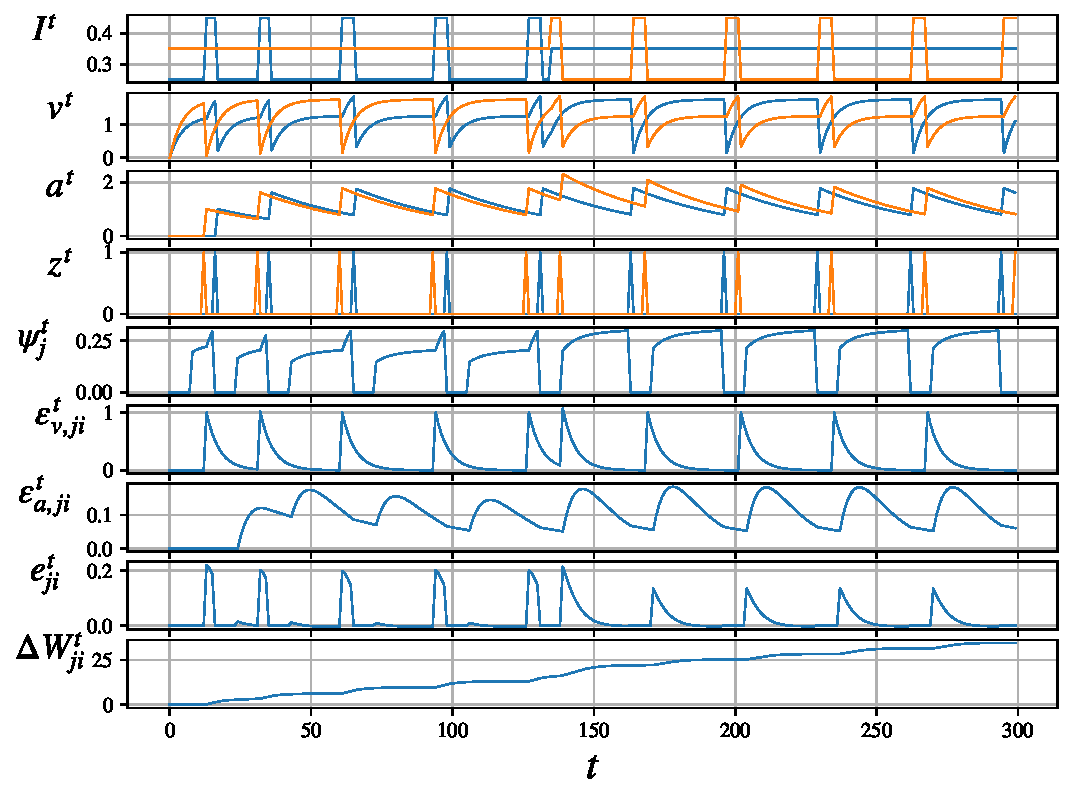
\includegraphics[width=0.8\linewidth]{alif}
  \end{figure}
\end{frame}

\begin{frame}{Methods -- STDP-ALIF}
  \begin{figure}[!ht]
    \centering
    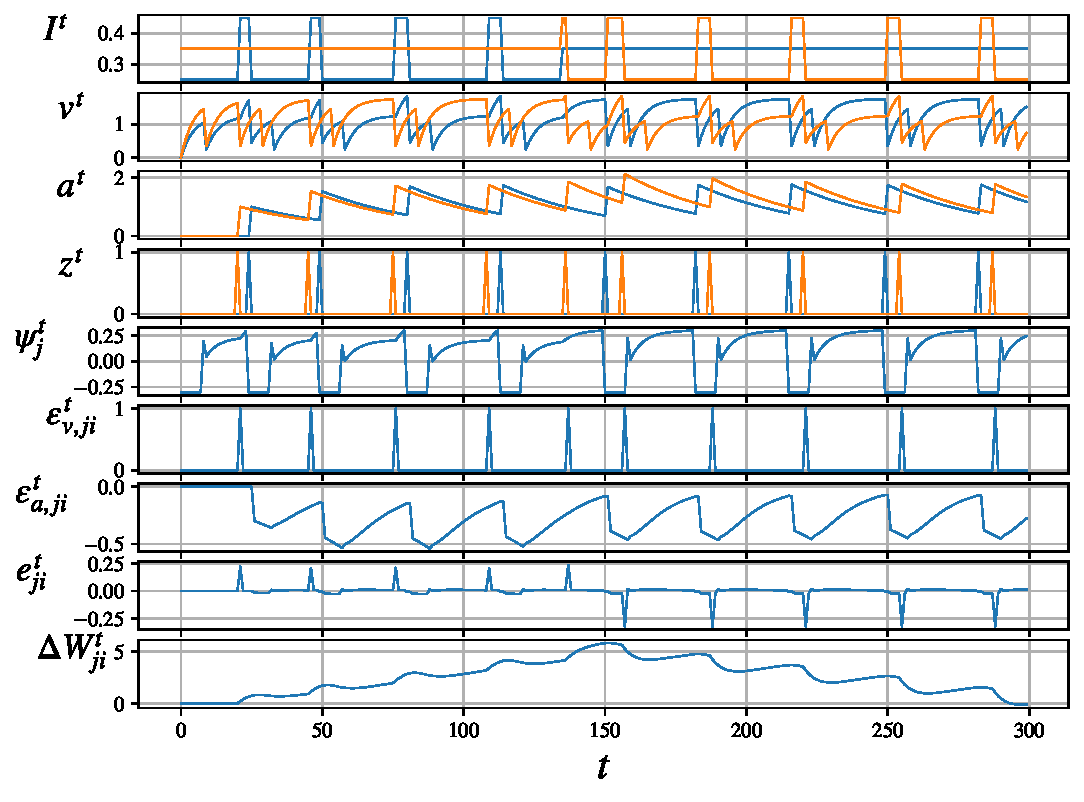
\includegraphics[width=.8\linewidth]{stdpalif}
  \end{figure}
\end{frame}
\begin{frame}{Methods -- Izhikevich}
  \begin{figure}[!ht]
    \centering
    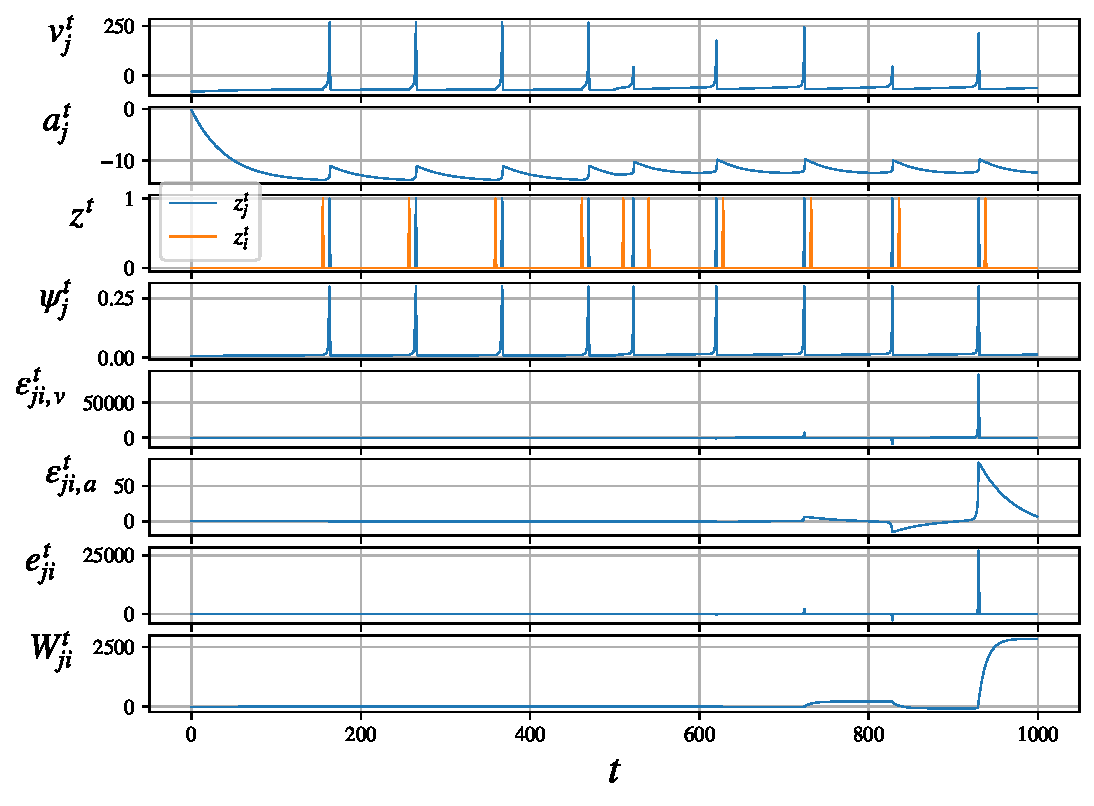
\includegraphics[width=0.8\linewidth]{demo_izh}
  \end{figure}
\end{frame}

\begin{frame}{Methods -- Izhikevich fixed}
  \begin{figure}[!ht]
    \centering
    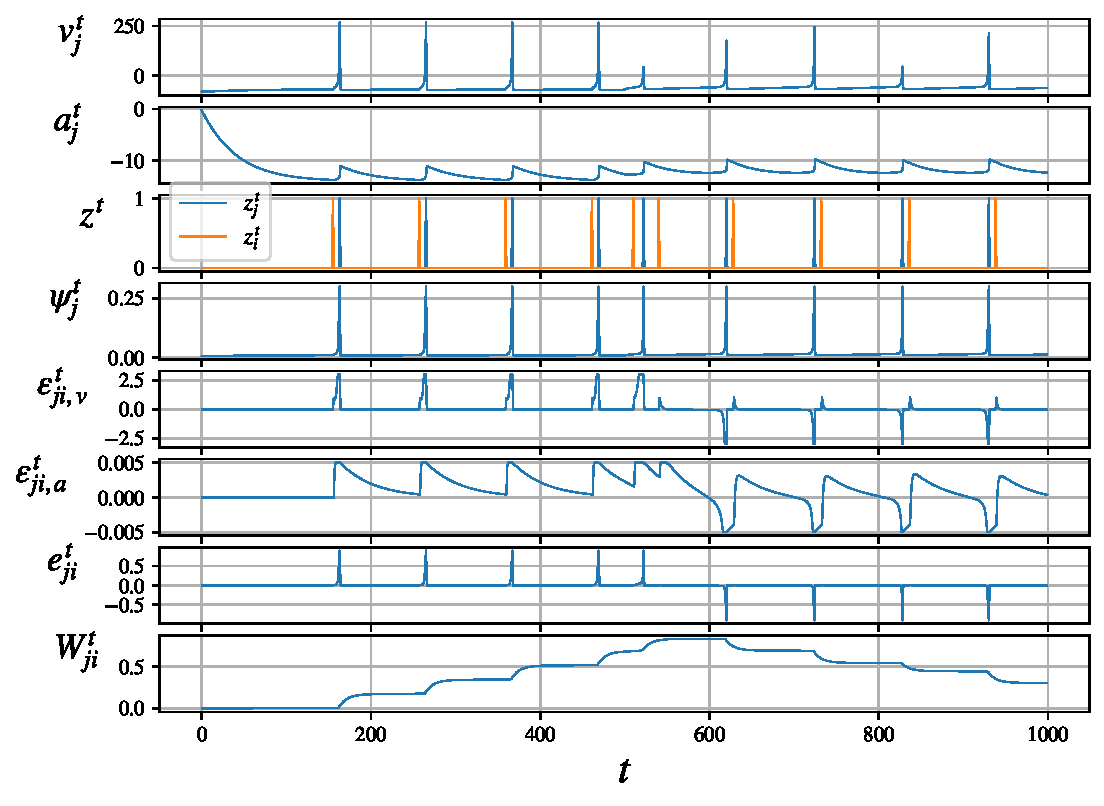
\includegraphics[width=0.8\linewidth]{demo_izh_corrected}
  \end{figure}
\end{frame}

\begin{frame}{Methods -- Multilayer}
  \begin{equation}\label{eq:ml_model}
        \mathbf{h}^t_{rj} = \begin{cases}
        M\left(\mathbf{h}_{rj}^{t-1}, \mathbf{z}_r^{t-1}, \mathbf{x}^t, \mathbf{W}_{rj}\right)       & \mbox{if } r = 1\\
        M\left(\mathbf{h}_{rj}^{t-1}, \mathbf{z}_r^{t-1}, \mathbf{z}_{r-1}^t, \mathbf{W}_{rj}\right) & \mbox{otherwise,}
        \end{cases}
        \end{equation}
        where $r \in [1\mathrel{{.}\,{.}}\nobreak R]$.

  \begin{figure}[!ht]
    \centering
    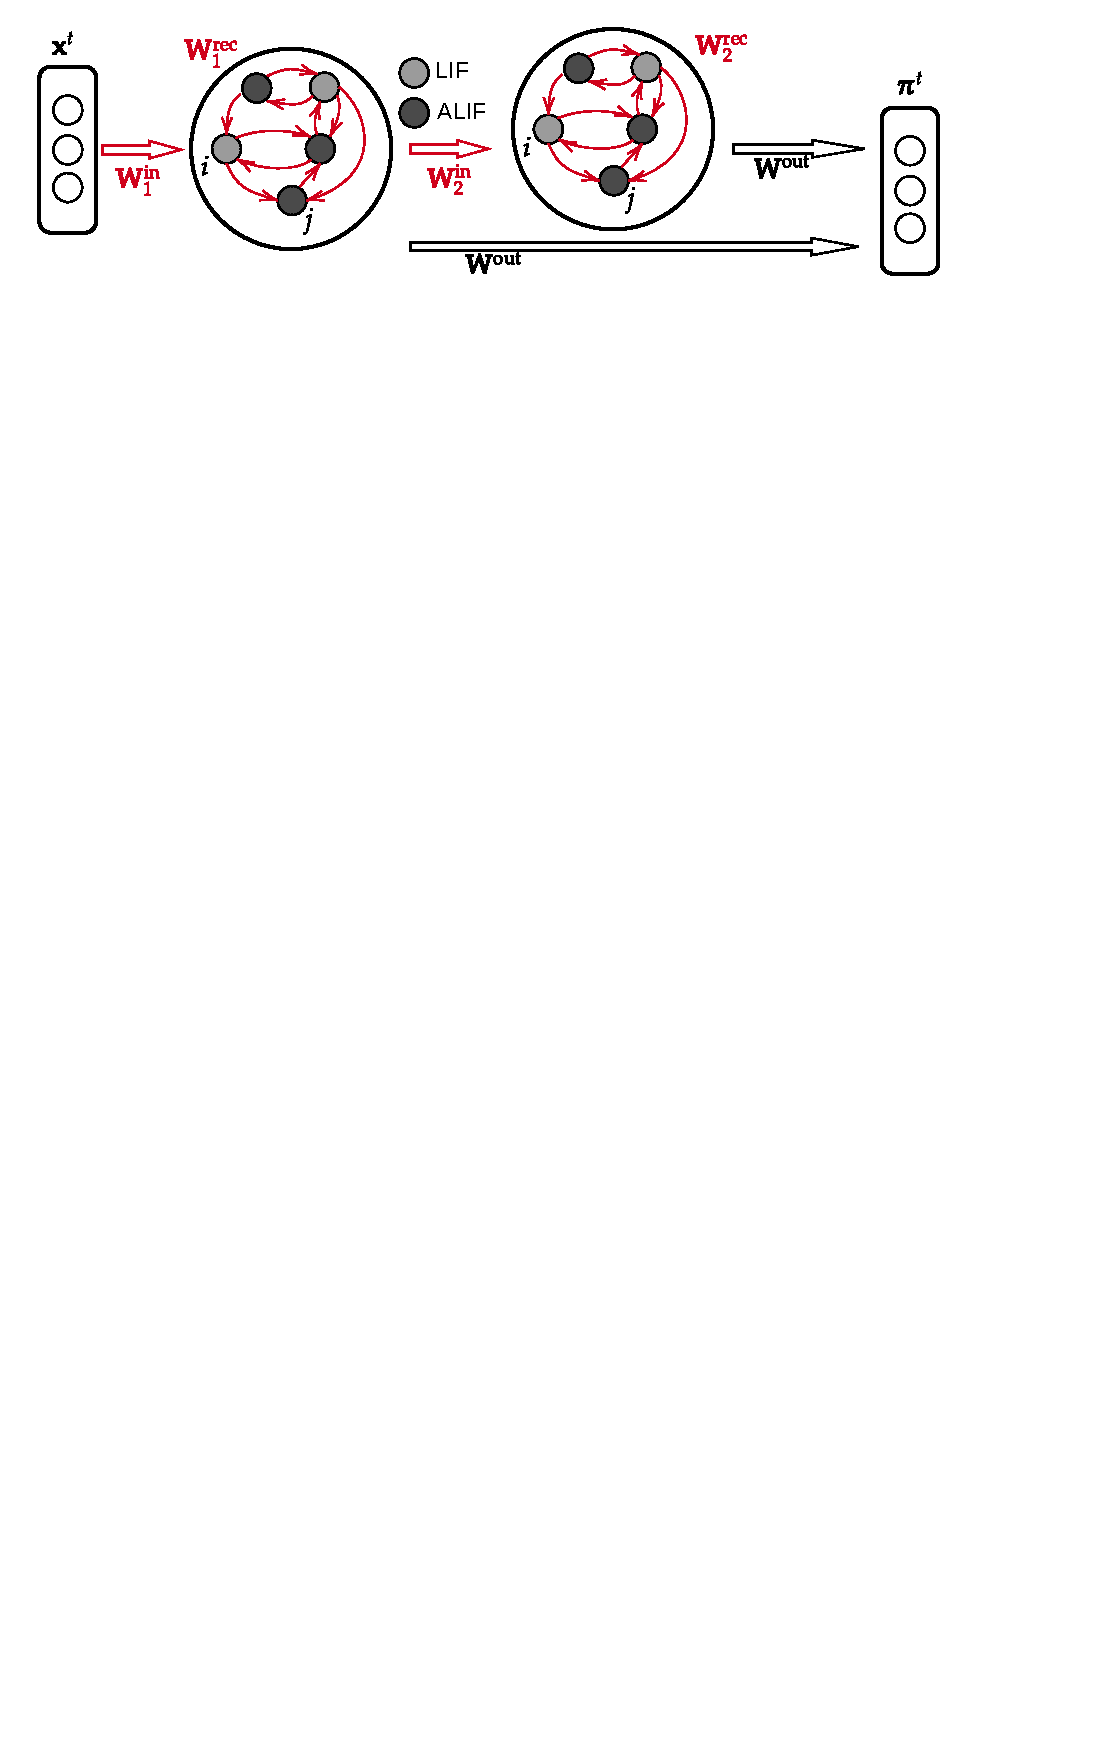
\includegraphics[trim=0 25cm 0 0, clip, width=\linewidth]{Multilayer}
  \end{figure}
\end{frame}

\begin{frame}{Methods -- Task}
  \begin{itemize}[label=--]
    \item Classify frame-wise phones from speech signals.
    \item There are 61 different class labels, and approximately 4000 speech sentences containing around 200-300 frames each.
    \item Speech is preprocessed into MFCCs (2--13) with their 1\textsuperscript{st} and 2\textsuperscript{nd} deltas, standardized per channel
  \end{itemize}
  \begin{figure}[!ht]
    \centering
    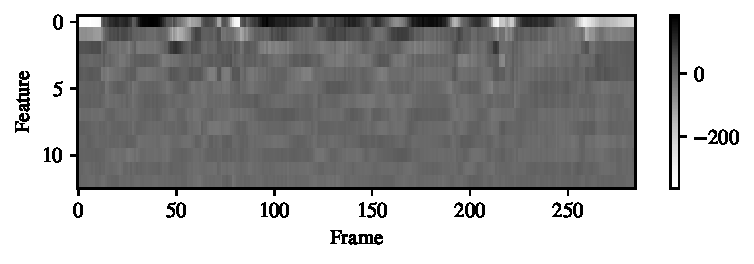
\includegraphics[width=\linewidth]{norm_mfcc}
  \end{figure}
  \begin{figure}[!ht]
    \centering
    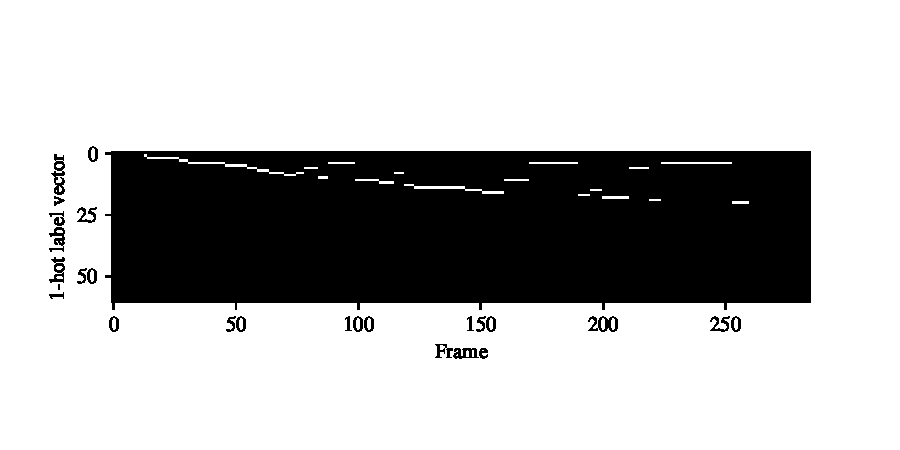
\includegraphics[width=\linewidth]{target}
  \end{figure}
\end{frame}

\begin{frame}{Methods -- Other settings}
  \begin{itemize}[label=--]
    \item Adam optimizer for e-prop
    \item Firing rate regularization
    \item L2 regularization
  \end{itemize}
\end{frame}

\section{Results}

\begin{frame}{Results -- Example}
  \begin{figure}[!ht]
    \centering
    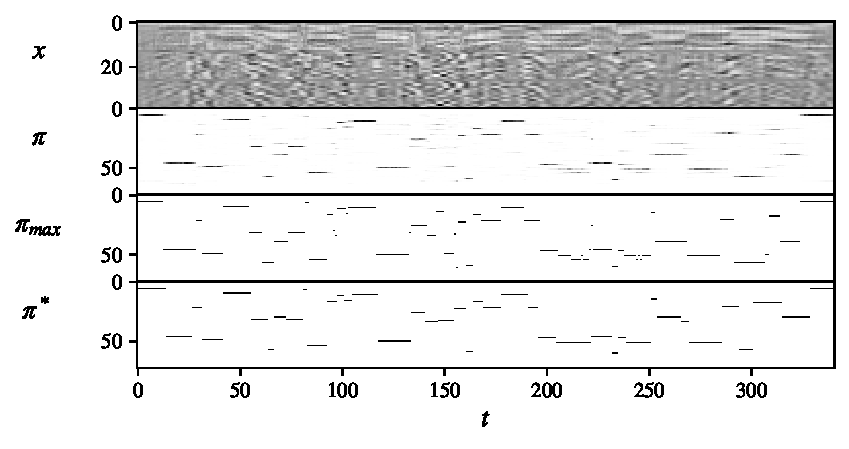
\includegraphics[width=\linewidth]{InOutPair}
  \end{figure}
\end{frame}

\begin{frame}{Results -- Accuracy per neuron type}
  \begin{figure}[!ht]
    \centering
    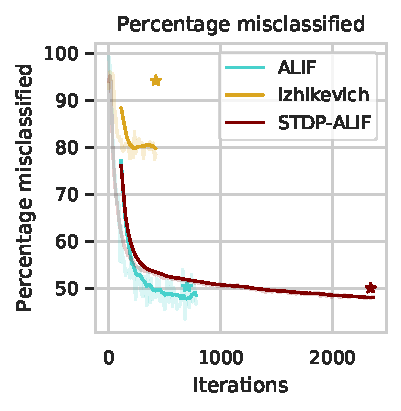
\includegraphics[width=0.5\linewidth]{percwrong}
  \end{figure}
  Test scores: ALIF = 50.3\%, STDP-ALIF = 50\%, Izhikevich = 94.2\%
\end{frame}

\begin{frame}{Results -- Cross-entropy per neuron type}
  \begin{figure}[!ht]
    \centering
    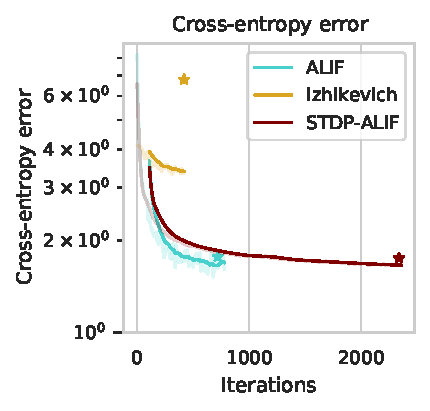
\includegraphics[width=0.6\linewidth]{crossentropy}
  \end{figure}
\end{frame}

\begin{frame}{Results -- Multi-layer effects}
  \begin{figure}[!ht]
    \centering
    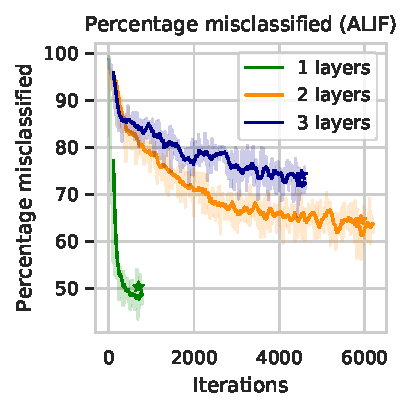
\includegraphics[width=0.6\linewidth]{ml-percwrong-ALIF}
  \end{figure}
\end{frame}

\begin{frame}{Results -- Multi-layer effects}
  \begin{figure}[!ht]
    \centering
    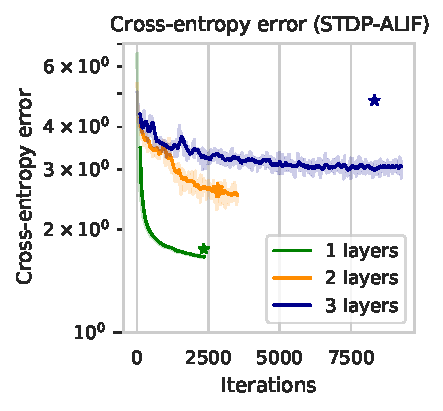
\includegraphics[width=0.6\linewidth]{ml-crossentropy-STDP-ALIF}
  \end{figure}
\end{frame}


\section{Discussion}
\begin{frame}{Discussion}
  \begin{itemize}[label=--]
    \item Izhikevich neuron unsuitable
    \item More layers = less efficient
    \item ALIF and STDP-ALIF contested\\$\rightarrow$ STDP inclusion slower but stabler and more accurate gradient descent
  \end{itemize}
\end{frame}

\begin{frame}{Discussion -- future research}
  \begin{itemize}[label=--]
    \item Smoothen output
    \item Distributed parameters
    \item Custom connectivity graphs
    \item Dynamic pruning and growing
    \item Synaptic delay
  \end{itemize}
\end{frame}

\begin{frame}{Conclusion}
  \begin{itemize}[label=--]
    \item Good trade-off between running cost and performance
    \item Interesting neurocomputational model
    \item More bioplausibility $\rightarrow$ easier in NC but not always better performance
    \item More research is needed on applying e-prop in other types of learning tasks, and many ideas exist that may improve performance
  \end{itemize}
\end{frame}

\end{document}
INTRODUCTION -- CONTEXT

For some historical context I want to start where the field of AI started; with the early goal of constructing systems that replicate ``intelligent behavior''.
One of the proposed methods was to use Perceptrons, which are simple units meant to emulate biological neurons.
This was in part inspired by Hebbian learning, which was a relatively new theoretical framework of biological learning.
In artificial neural networks (ANNs), a network of these neurons can learn simple tasks.
ANNs became more popular when the backpropagation learning method allowed ``deeper'' ANNs, which have multiple stacked layers, to learn more complex tasks.
In the last decade, deep learning became a dominant field within AI, and can now perform as well as humans at some narrowly defined tasks.

INTRODUCTION -- RELEVANCE

However, a major drawback of deep learning is that it consumes a lot of data and energy, which is increasingly bottlenecking its progress.
This is a clear indication that AI has gone astray in its initial motivation to draw inspiration from human cognition.
The human brain consumes approximately 20W, while some deep learning models cost millions of USD in energy to train.
This is caused by fundamental differences between deep learning and the human brain.

In the human brain, communication between neurons is binary in the form of action potentials propagating along an axon.
Information is contained in the temporal pattern of this so-called spike train.
In deep learning, communication occurs at every propagation cycle, and the information is contained in the floating-point values.
This essentially means that in DL, all neurons fire all the time.

A second difference is the learning algorithm.
In deep learning, this happens by backpropagation, or backpropagation through time in recurrent networks, which require a biologically implausible backward pass from the last layer to earlier layers.
Every connection weight in the network is moved in the negative direction of the error gradient.
In the human brain, there is no such backward pass.
Instead, synapses get stronger or weaker depending on biological learning signals, such as neurotransmitters.

INTRODUCTION -- SNNs

Spiking neural networks are a next step in the direction of biological plausibility.
In an SNN, neurons fire binary spikes instead of propagating floating-point values.
Since spikes cannot be integrated, the gradient of the error cannot directly be calculated.
This means that backpropagation is harder to implement.
There are many other learning algorithms for SNNs, but most do not compete well with human learning or deep learning.

INTRODUCTION -- NEUROMORPHIC COMPUTING

SNNs are particularly useful in the upcoming field of neuromorphic computing, in which very-large-scale integration systems are used to implement neural systems.
A key difference with ANNs is that neuromorphic systems are physical embeddings in an analog medium, rather than an emulation in a digital system.

This means that neuromorphic systems are not based on Von Neumann architectures, in which central processing and memory is separated, but have colocalized memory and computation.
The lack of a separate memory also precludes the use of backpropagation, but other SNN learning algorithms may still be used.

SNNs embedded in neuromorphic systems are extremely fast and energy efficient compared to emulated SNNs.

However, their learning algorithms must be local and online.
``Local'' means that a neuron can only access information that is directly communicated to it, or directly available in its own unit.
``Online'' means that only information available at the current time step can be accessed.
The human brain also has these natural constraints, and so it is a logical step to be re-inspired by the human brain.

INTRODUCTION -- BIOLOGICAL LEARNING

I have already alluded to Hebbian learning, which is a simple biological learning theory best described as ``cells that fire together, wire together''.
However, this inevitably leads to runaway excitation, because this is a positive feedback loop.
Spike-timing-dependent plasticity is a refined version of Hebbian learning, in which a connection gets stronger if a postsynaptic neuron fires right after a presynaptic neuron, because this suggests that the presynaptic neuron had a causal contribution to the postsynaptic spike.
And if it is the other way around, there was no causal contribution and the synapse weakens.

However, to allow a neural network to learn tasks, there needs to be a learning signal that indicates a desired response to an input.
In psychology, classical conditioning is a clear example.
The inclusion of this learning signal to Hebbian learning is called three-factor Hebbian learning, and to STDP it is called reward-modulated STDP.
Neurotransmitters such as dopamine and acetylcholine are examples of learning signals in biological learning.

However, if a learning signal arrives with some delay after the behavior, it should still work.
And when a learning signal occurs, how can one know which synapses had fired at the time of the behavior, and contributed to it?
This problem of assigning credit to spikes in the past can be solved by using eligibility traces.

Eligibility traces leave an explicit afterimage after a spike, which persists for much longer time spans than the chemical traces that elicited the spike itself.
When such a fading eligibility trace is followed by a learning signal, synaptic plasticity is still induced.
This has been shown to occur in the human brain.
Learning algorithms using eligibility traces have also shown some successes in training SNNs using R-STDP.

INTRODUCTION -- ELIGIBILITY PROPAGATION (1/2)

One of these is called eligibility propagation, or e-prop.
There is a mathematical connection to backpropagation, but the algorithm itself is biologically plausible, because it adheres to the local and online constraints.

It is applicable to any connectivity topology, and multiple neuron models can be used.
Different neuron models produce spikes using different equations.

E-prop is suitable for very-large scale integration systems.
And finally, it performs competitively with LSTMs on phone classification.
A phone is a technical word for speech sound.

INTRODUCTION -- ELIGIBILITY PROPAGATION (2/2)

However, only the ALIF neuron type has been examined in the e-prop framework.
This ALIF neuron does not show STDP-like behavior.
New research has suggested that the STDP-LIF and Izhikevich neurons do display STDP

INTRODUCTION -- THIS RESEARCH

(literal)

===============================================================================

METHODS -- TECHNICAL FRAMEWORK (E-PROP)
